
\documentclass[12pt]{article}
\usepackage{graphicx}
\graphicspath{ {./images/} }
\usepackage{epsfig}
\usepackage{amsmath,amsthm}
\usepackage{listings}
\usepackage[dvipsnames]{xcolor}

\newtheorem{lemma}{Lemma}
\newtheorem{theorem}{Theorem}


\usepackage{titlesec}
\titleformat{\section}
{\normalfont\Large\bfseries}{Question~\thesection:}{1em}{}

\newlength{\toppush}
\setlength{\toppush}{2\headheight}
\addtolength{\toppush}{\headsep}


\def\subjnum{Comp 160}
\def\subjname{Algorithms}


\def\doheading#1#2#3{\vfill\eject\vspace*{-\toppush}
  \vbox{\hbox to\textwidth{{\bf} \subjnum: \subjname \hfil Erli Cai}
    \hbox to\textwidth{{\bf} Tufts University, Fall 2020 \hfil#3\strut}
    \hrule}}


\newcommand{\htitle}[1]{\vspace*{1.25ex plus 1ex minus 0ex}
\begin{center}
{\large\bf #1}
\end{center}} 






\begin{document}
\doheading{2}{title}{Homework 01}



\section{}
(a) Can't tell which algorithm is faster, since big O notation only tells us the upper bound each algorithm.\\

\noindent(b) R1 is faster. Algorithm 1 takes linear time at most while Algorithm 2 takes at least quadratic time.\\


\noindent(c) Can't tell which algorithm is faster, Since R2 could run in $\theta(1)$ time, which us faster than R1 or it could run in $\theta (n^2)$ time which is slower than R1.\\


\noindent(d) R1 runs faster. Algorithm 1 takes linear time at most while Algorithm 2 takes exactly quadratic time.\\

\pagebreak

\section{}
$f(n) = 3n^2 + 10n +729$\\

\begin{flalign*}
(a) f(n) &\leq 3n^2 + 10n + 729n \quad\mbox{ when } n \geq 729 &&\\
            &= 3n^2 + 739n &&\\
            &\leq 3n^2 + 739n^2  \quad\mbox{ when } n \geq 739&&\\
            &= 742n^2 = O(n^2) 
\end{flalign*}

\begin{flalign*}
(b) f(n) & \leq 742n^2 \quad\mbox{proved in part(a)} &&\\
&\leq 742n^3 \quad\mbox{ when } n \geq 742&&\\
&= O(n^3) &&
\end{flalign*}

\begin{flalign*}
(c) f(n) & \geq 3n^2 + 10n &&\\
&\geq 10n \quad\mbox{ since } n^2 \geq 0&&\\
&= \Omega(n) &&
\end{flalign*}

\begin{flalign*}
(c) f(n) & \geq 3n^2 + 10n &&\\
&\geq 3n^2 \quad\mbox{ when } n \geq 0&&\\
&= \Omega(n^2) &&
\end{flalign*}
\\

\noindent(d) $O(n^2)$ and $\Omega(n^2)$ are better bounds.\\
This is because they have a smaller range. That is to say, every function which is $O(n^2)$ is $O(n^3)$ but not vice versus.\\
For example, $3n^3$ is $O(n^3)$ but not $O(n^2)$

\pagebreak


\section{}

(a)\\
 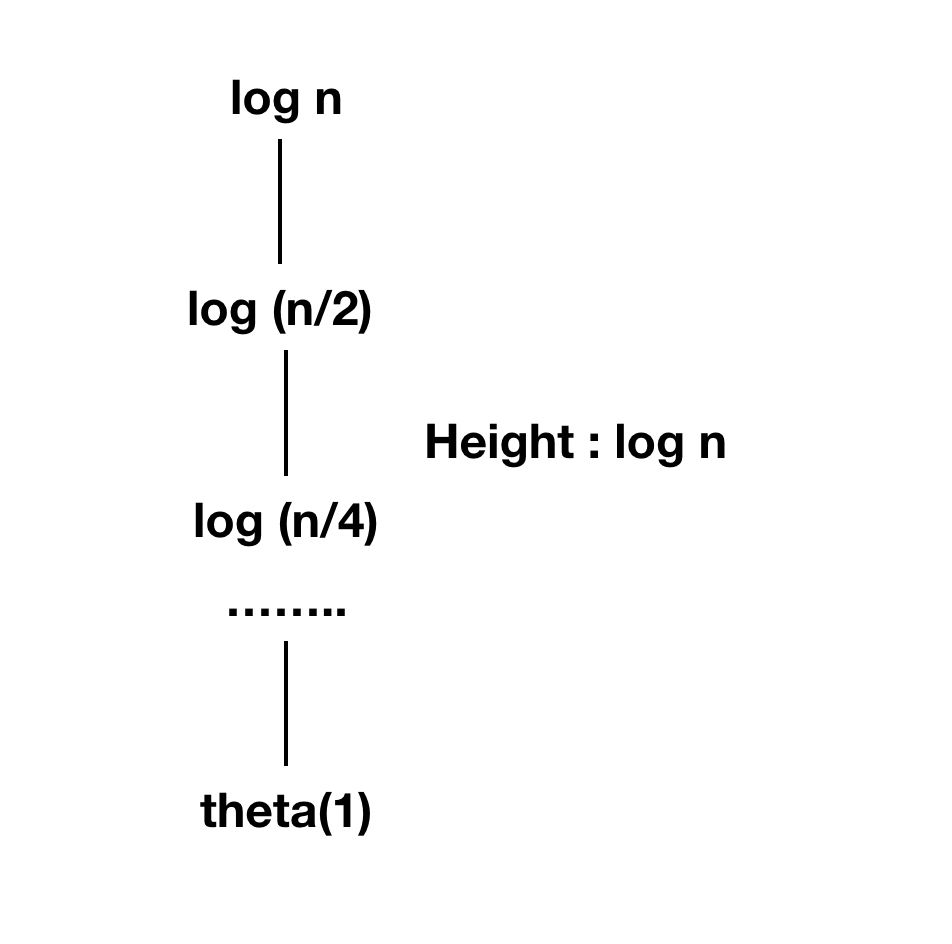
\includegraphics[width=80mm]{Screenshot1}\\
Level sum shrinks and the max level sum is at root \\
$H(t) \leq height \times \mbox{max(level sum)} = log(n) \times log(n) = O(log^2(n))$\\


\noindent(b)\\
Guess: Lower bound is $O(log^2(n))$ \\
Base case: $H(2) = \Theta(1) = d > c log^2(2) = c \Longleftrightarrow 0 < c < d$ \\
Induction hypothesis: $H(n) > c log^2(n)$ for all $n < k$  \\
Induction step: 
\begin{flalign*}
H(n) &= H(\frac{n}{2}) + \log(n)  &&\\
       &\geq c log^2(\frac{n}{2}) + log(n) \\
       & = c (log(n)-log(2))^2 + log(n)\\
       & = c (log^2(n)-2log(n)log(2) +log^2(2) ) + log(n)\\
       & = clog^2(n) + clog^2(2)+ log(n)\times(1-2clog(2))\\
       & \geq clog^2(n) \mbox{ when } 1-2clog(2) > 0  \Longleftrightarrow  0 < c < \frac{1}{2log(2)}\\
       & = \Omega(log^2(n))
\end{flalign*}


\noindent(c)\\
$a = 1, b = 2, \quad f(n) = \log n$\\
$n^{\log_ba} = n^{\log_2 1} = n^0 = 1$ so $f(n) = \Theta(n^{\log_ba}\log n)$\\
Applying master method, we know that, $H(n) = \Theta(f(n) \log n) =  \Theta(\log^2 n)  $\\




\noindent(d)\\
The bounds match.\\
I would prefer using master method on this question, since it can solve the upper bound and lower bound simultaneously in just a few lines.


\pagebreak


 \textcolor{red}{ 
 $G_{t:t+n} = R_{t+1} + \gamma R_{t+2}+..+\gamma^{n-1} R_{t+n} + \gamma^nQ_{t+n-1}(S_{t+n})$\\
 }\\
 
   \textcolor{red}{ 
  $R_T = 0$ for all T except terminal state
 }\\
 
 
  \textcolor{red}{ 
  $Q_{t+n}(S_{t}) = Q_{t+n-1}(S_{t})+\alpha [G_{t:t+n} -Q_{t+n-1}(S_{t}) ]$\\
 }
 
 


\end{document}


